\chapter{Problema}
La agricultura urbana es un concepto que integra dos actores importantes en el desarrollo social : el campo y la ciudad. Surge con el objetivo de potenciar los escenarios comunitarios de la ciudad, la recuperación de los recursos naturales y la generación de actividades que inciten la producción agro-cultural , logrando un encadenamiento que favorece las dimensiones ecológicas, políticas, sociales y económicas de los individuos.Es por eso que los retos de las ciudades contemporáneas obligan a integrar
los proyectos de cultivos urbanos dentro de un proceso
general de rehabilitación urbana ecológica. \cite{moran2010agricultura} \\

Esta integración implica que las personas  involucradas en un primer plano,tales como, los agricultores urbanos y los poseedores de cultivos pequeños o medianos se acojan a los quehaceres y deberes para la manutención, sostenibilidad y sustento de su cultivo. Sin embargo, en el marco de urbanidad es difícil adaptarse a conductas y comportamientos propios de una locación agrícola común. Las tareas de riego, abonado y recepción de luz natural muchas veces se incumplen cada tanto por cuestiones ajenas a los individuos. La misma estructura social y la cotidianidad de una persona que reside y se desenvuelve en una ciudad incide en este apartado.\\

Una de las tareas más importantes para el cuidado de un huerto urbano es el monitoreo constante de estas mismas variables que están en juego en el desarrollo de una planta, factores como la luz, la humedad del suelo y la calidad del mismo, son elementos difíciles de monitorear pero que representan factores vitales para el desarrollo de una planta. En muchas ocasiones este proceso resulta complejo, principalmente por el hecho de no contar con el tiempo suficiente y la infraestructura para lograr un monitoreo eficaz, por ello se plantea en el presente documento una posible solución para que la agricultura urbana comience no a presentar mas trabajo, sino por el contrario sea una opción fácil y rápida, además que contribuya a que las ciudades recuperen algo de la calidad de aire que puede llegar a significar la agricultura urbana.

\begin{figure}[th!]
	\centering
	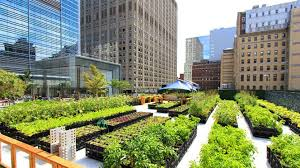
\includegraphics[width=0.7\linewidth]{proyecto/imgs/agriculturaurbana}
	\caption{Agricultura urbana}
	\label{fig:rup}
\end{figure}
\section{Aspecto económico}
Para abordar el impacto económico que puede llegar a tener la agricultura urbana en nuestro país, se tomará como ejemplo el caso de Cuba, un país que dependía en gran medida del campo socialista Europeo, sin embargo al momento de su caída, Cuba afrontó un momento de profunda crisis económica, que generó una fuerte escasez de alimentos, tanto los que provenían de las importaciones como los de la producción nacional. \\

La búsqueda de soluciones emergentes a toda esta situación promovió que se desarrollaran diversas soluciones, con una marca local, entre ellas la \textbf{agricultura urbana, como alternativa para incrementar la disponibilidad de alimentos}, permitiendo así un acceso efectivo a los alimentos y además de ello la superación de la crisis.\cite{houtart2004globalizacion}\\

Se destaca además que el uso de estrategias de producción eficientes y la especialización de las plantas de un cultivo, generan un alto valor económico en las sociedades\cite{civittolo2012extension} . Ahora bien, el que una persona disponga de un huerto casero en la urbe presenta beneficios económicos para el, tales como el ahorro en productos del sector primario que se acostumbran a comprar día a día. En adición, puede presentarse la oportunidad del nacimiento de microempresas bajo la consigna de agricultura urbana.

\section{Aspecto social}
El primer beneficio que las personas vinculadas a la agricultura urbana pueden evidenciar es la mejora en su autoestima, esto se debe principalmente a que se sienten importantes y útiles a los demás, no solo cuando obtienen el producto final de la planta, sino que también cuando comparten sus conocimientos con otras personas que realizan la misma actividad.

Las personas con problemas de discapacidades físicas o mentales, sienten una mejoría consigo mismos y con las personas que los rodean, la sensación de utilidad a la sociedad es una parte vital para su evolución, ademas de que no solo personas con discapacidades se ven beneficiadas, personas en cárceles adquieren la sensación de retribución a la sociedad de algo del daño hecho.

Socialmente la agricultura urbana impacta la calidad de la alimentación, la obtención de ingresos no imputables( lo que se consume pero no se paga con dinero), además una adopción de un estilo de vida de producción agrícola, puede significar relaciones sociales propias de la vida del campo, acoplándolas con algunos comportamientos propios de la vida en la ciudad   

\section{Aspecto ambiental}
"se estima que unos 800 millones de habitantes de ciudades de todo el mundo participan en actividades relacionadas con la agricultura urbana y periurbana, que les producen alimentos y generan ingresos. Una combinación de datos de censos nacionales, encuestas a hogares y proyectos de investigación señalan que hasta dos tercios de los hogares urbanos y periurbanos participan en la agricultura. Una gran parte de los productos de la agricultura urbana se destinan al consumo propio, mientras que los excedentes ocasionales se venden en el mercado local" (AQUI VA UNA CITA Y CURSIVA Y TODO ESO)

Estas estadísticas a nivel mundial, reflejan la preocupación y el deseo de tener un medio de producción más sostenible. La agricultura urbana es una clara alternativa, dado que tiene un gran número de beneficio no solo económicos, puesto que minimiza los costos de producción y envío de alimentos a centros urbanos, que eventualmente aumentan proporcionalmente a la distancia que deba recorrer los productos para llegar a su destino, sino que también conlleva beneficios medio ambientales, en una sociedad acostumbrada a ciudades de cemento, grandes edificios y pocas zonas verdes, la inserción de la naturaleza, no solo en parques y jardines, sino en huertas, ayuda a generar zonas verdes, en terrenos que actualmente están vacíos, además de recuperar el ciclo del metabolismo urbano, conformado por el agua, la energía y la materia.

Por otro lado, puede ser visto como una posibilidad de recuperar variedades de flora y fauna locales, protegiendo y aumentando la biodiversidad en las ciudades.El manejo ambiental que maneja este tipo de agricultura nos da un amplio espectro, principalmente porque hay que aplicar una contundente utilización de residuos orgánicos e inorgánicos (elaboración de abonos, utilización como contenedores o como medios de cultivo)

\begin{figure}[th!]
	\centering
	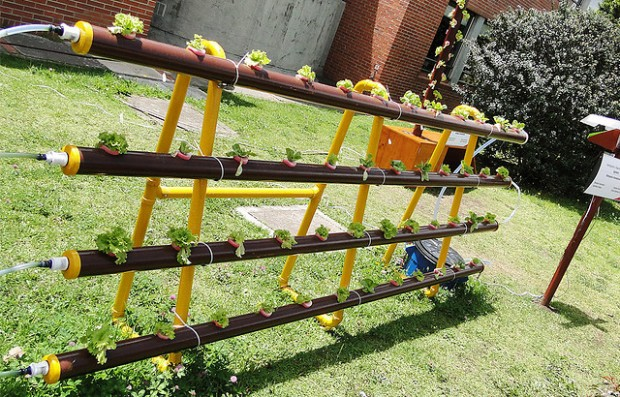
\includegraphics[width=0.7\linewidth]{proyecto/imgs/ag1}
	\caption{Agricultura urbana}
	\label{fig:rup}
\end{figure}

\section{Aspecto cultural}
El daño al planeta generado por la producción de CO2 en las ciudades, y el reducido número de zonas verdes capaces de absorber estas partículas, han sido temas difíciles de manejar en la actualidad. Las huertas y jardines urbanos son una clara solución y poco a poco ha generado conciencia en los habitantes, esto se puede ver reflejado por ejemplo en que Bogotá cuenta con el jardín vertical mas grande del mundo. Santalaia, un edificio residencial con más de 115 mil plantas distribuidas estratégica mente en 3.117 metros cuadrados, el edificio luce un revestimiento verde, que alude al ambiente de una selva tropical.

Santalaia es capaz de producir el oxígeno que necesitan más de 3 mil personas al año, incluso, ayuda a procesar 2 mil toneladas de gases nocivos y más de 400 kilogramos de polvo que genera la polución. Si se incentiva la creación de jardines y huertas urbanas como el caso anterior, es evidente el cambio positivo que se produce en una ciudad. 

Además, el uso de dispositivos móviles para controlar los cuidados de las plantas, motivará mas a las personas a cultivar su propio jardín, ayudando a las personas que no disponen de mucho tiempo para cuidarlos a mantener las plantas a salvo y así generar una conciencia ecológica en los habitantes de las ciudades.

\begin{figure}[th!]
	\centering
	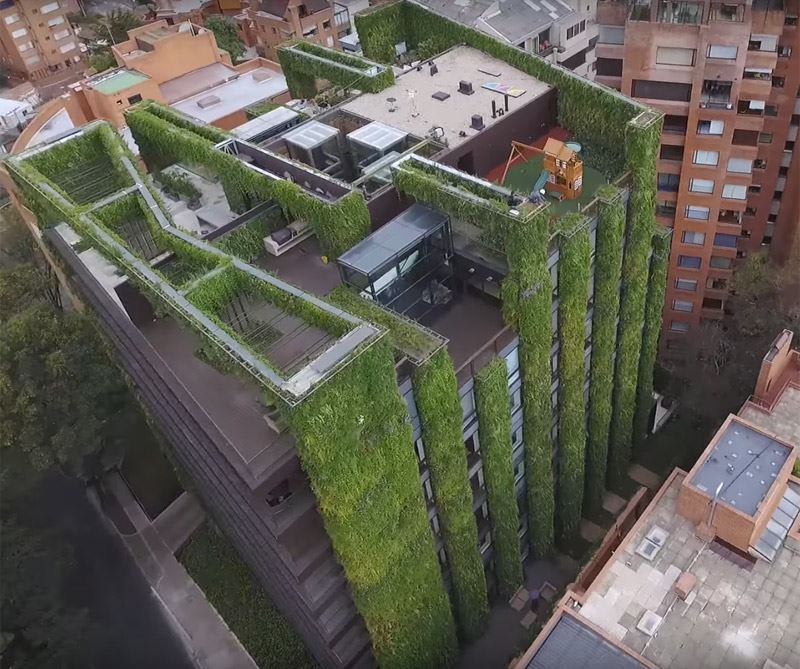
\includegraphics[width=0.7\linewidth]{proyecto/imgs/cultu}
	\caption{Edificio Santalaia}
	\label{fig:rup}
\end{figure}
